\documentclass[12pt, titlepage]{article}

\usepackage{booktabs}
\usepackage{tabularx}
\usepackage{hyperref}
\hypersetup{
    colorlinks,
    citecolor=black,
    filecolor=black,
    linkcolor=red,
    urlcolor=blue
}
\usepackage[round]{natbib}
\usepackage{longtable}
%% Comments

\usepackage{color}

\newif\ifcomments\commentstrue %displays comments
%\newif\ifcomments\commentsfalse %so that comments do not display

\ifcomments
\newcommand{\authornote}[3]{\textcolor{#1}{[#3 ---#2]}}
\newcommand{\todo}[1]{\textcolor{red}{[TODO: #1]}}
\else
\newcommand{\authornote}[3]{}
\newcommand{\todo}[1]{}
\fi

\newcommand{\wss}[1]{\authornote{blue}{SS}{#1}} 
\newcommand{\plt}[1]{\authornote{magenta}{TPLT}{#1}} %For explanation of the template
\newcommand{\an}[1]{\authornote{cyan}{Author}{#1}}

%% Common Parts

\newcommand{\progname}{ProgName} % PUT YOUR PROGRAM NAME HERE
\newcommand{\authname}{Team \#, Team Name
\\ Student 1 name
\\ Student 2 name
\\ Student 3 name
\\ Student 4 name} % AUTHOR NAMES                  

\usepackage{hyperref}
    \hypersetup{colorlinks=true, linkcolor=blue, citecolor=blue, filecolor=blue,
                urlcolor=blue, unicode=false}
    \urlstyle{same}
                                

\usepackage{graphicx}

\begin{document}

\title{Verification and Validation Report: \progname} 
\author{\authname}
\date{\today}
	
\maketitle

\pagenumbering{roman}

\section{Revision History}

\begin{tabularx}{\textwidth}{p{3cm}p{2cm}X}
\toprule {\bf Date} & {\bf Version} & {\bf Notes}\\
\midrule
03/10/2025 & 0.1 & Rev0\\
\ldots & \ldots & \ldots\\
\bottomrule
\end{tabularx}

~\newpage

\section{Symbols, Abbreviations and Acronyms}


Refer to the
\href{https://github.com/PlutosCapstone/Plutos/blob/main/docs/SRS/SRS.pdf}{Software
Requirements Specification (SRS)} document for the list of abbreviations and
acronyms (Section 1.3) and the list of symbolic constants (Section 10).


In addition, the following abbreviations are used in this document:\\

\renewcommand{\arraystretch}{1.2}
\begin{table}[h!]
\caption{Symbols, Abbreviations, and Acronyms}
\begin{tabularx}{\textwidth}{l l}
  \toprule		
  \textbf{symbol} & \textbf{description}\\
  \midrule 
  V\&V & Verification and Validation\\
  UI & User Interface\\
  OCR & Optical Character Recognition\\
  SQL & Structured Query Language\\
  GDPR & General Data Protection Regulation\\
  \bottomrule
\end{tabularx}
\end{table}

\newpage

\tableofcontents

\listoftables %if appropriate

\listoffigures %if appropriate

\newpage

\pagenumbering{arabic}

This document reports the results of the Verification and Validation (V\&V)
process for the \progname software. The V\&V plan is documented in the
\href{https://github.com/PlutosCapstone/Plutos/blob/main/docs/VnVPlan/VnVPlan.pdf}{Verification
and Validation Plan} document. 

\section{Functional Requirements Evaluation}

The functional system tests can be found in Section 4.1 of the
\href{https://github.com/PlutosCapstone/Plutos/blob/main/docs/VnVPlan/VnVPlan.pdf}{Verification
and Validation Plan} document. These tests are all performed manually.

\begin{table}[h!]
\centering
\caption{Functional Requirements Evaluation}
\begin{tabularx}{\textwidth}{>{\centering\arraybackslash}X >{\centering\arraybackslash}X >{\centering\arraybackslash}X}
  \toprule
  \textbf{Test ID} & \textbf{Pass/Fail} & \textbf{Comments} \\
  \midrule
  test-UAM-1 & Pass &  \\
  test-UAM-2 & Pass &  \\
  test-UAM-3 & Pass &  \\
  test-UAM-4 & Fail & Not yet implemented \\
  test-UAM-5 & Pass &  \\
  test-UAM-6 & Pass &  \\
  \midrule
  test-IP-1 & Pass & \\
  test-IP-2 & Pass & \\
  test-IP-3 & Fail & Not yet implemented \\
  \midrule
  test-MIS-1 & Pass & \\
  \midrule
  test-DM-1 & Pass & \\
  test-DM-2 & Pass & \\
  \midrule
  test-RS-1 & Pass & \\
  test-RS-2 & Pass & \\
  test-RS-3 & Pass & \\
  \midrule
  test-FT-1 & Fail & Not yet implemented \\
  test-FT-2 & Pass & \\
  test-FT-3 & Fail & Not yet implemented \\
  \bottomrule
\end{tabularx}
\end{table}

The User Account Management tests evaluate the core functionalities related to user 
account creation, login, logout, updates, authorization access, and password reset. Inputs 
for these tests typically consist of user-provided data such as names, emails, passwords, 
and session information. The expected outputs include confirmation messages and access to 
the user dashboard, with a pass being defined by the successful execution of each function 
without errors, ensuring a seamless user experience.

The Image Processing tests assess the application's ability to handle image uploads, 
previews, and file size limitations. Inputs for these tests include various image files, 
while the outputs are the successful display of uploaded images and adherence to file size 
constraints. A pass is determined by the system's ability to process the images correctly 
and provide appropriate feedback to the user.

The Manual Expense Input test assesses the application’s ability to handle manual 
input of expenses. The input for this test involves user-entered financial data, while the 
output is the successful recording and display of the entered expenses. A pass is determined 
by the system's ability to accurately capture and reflect the user's input without any 
discrepancies.

The Database Management tests evaluate the application's functionality in managing and processing
user data. Inputs for these tests consist of various data entries related to user expenses 
and financial records. The expected outputs are the correct storage and retrieval of this 
data, with a pass being defined by the system's ability to manage data effectively and 
provide accurate results when queried.

The Item Recognition and Categorization tests focus on the application's capability to generate reports based 
on user data. Inputs for these tests include user financial data and parameters for report 
generation. The outputs are the generated reports that summarize spending trends and 
financial insights. A pass is achieved when the reports are accurately produced and reflect 
the correct data as per user specifications.

The Financial Tracking tests are designed to evaluate the application's capabilities in 
tracking spending history, setting budgets, and notifying users when they approach their 
budget limits. Inputs for these tests consist of user-generated financial data, such as 
expenses and budget parameters. The outputs include visual representations of spending 
trends, budget tracking features, and notifications. A pass for these tests is achieved 
when the application accurately reflects the user's financial data and provides timely 
alerts, ensuring effective financial management for users.

\section{Nonfunctional Requirements Evaluation}

The nonfunctional system tests can be found in Section 4.2 of the
\href{https://github.com/PlutosCapstone/Plutos/blob/main/docs/VnVPlan/VnVPlan.pdf}{Verification
and Validation Plan} document. \textbf{Tests without comments are performed as
described in the plan.}


\begin{longtable}{>{\centering\arraybackslash}p{0.2\textwidth} >{\centering\arraybackslash}p{0.2\textwidth} >{\centering\arraybackslash}p{0.5\textwidth}}
  \caption{Nonfunctional Requirements Evaluation}\\
    \toprule
    \textbf{Test ID} & \textbf{Pass/Fail} & \textbf{Comments} \\
    \midrule
    test-ACC-1 & Pass &
    \href{https://github.com/PlutosCapstone/Plutos/tree/main/src/server/tests/imageProcessing/data/categorization/receipt_items_output.csv}{Actual
    output}; accuracy is 47/57 = 82.46\%, which meets the threshold of
    \textit{CATEGORIZATION\_ACCURACY}\%. Test can be found
    \href{https://github.com/PlutosCapstone/Plutos/blob/main/src/server/tests/imageProcessing/test_categorization.py}{here}.
    \\
    test-ACC-2 & Pass & By manually comparing the input
    \href{https://github.com/PlutosCapstone/Plutos/tree/main/src/server/tests/imageProcessing/data/parsing/input}{
    (set of receipt images)} with the
    \href{https://github.com/PlutosCapstone/Plutos/tree/main/src/server/tests/imageProcessing/data/parsing/input}{resulting
    output}, and calculating the accuracy as descripted in the V\&V Plan,
    current accuracy is ~80\%, which meets the threshold of \textit{OCR\_ACCURACY}\%.
    \begin{itemize}
      \item \textit{foodbasics\_1.jpg}: 13.5/15 = 90\%
      \item \textit{foodbasics\_2.jpg}: 7/9 = 77.78\%
      \item \textit{walmart\_1.jpg}: 7/10 = 70\%
      \item \textit{costco\_1.jpg}: 18.5/23 = 76.09\%
      \item Overall accuracy: 46/57 = 80.70\%
    \end{itemize}\\
    test-ACC-3 & Pass &  \\
    test-ACC-4 & Pass &  \\
    test-ACC-5 & Pass &  \\
    \midrule
    test-PERF-1 & Pass &  \\
    test-PERF-2 & Pass &  \\
    test-PERF-3 & Fail & Load testing has not yet been performed \\
    \midrule
    test-USAB-1 & Pass & Testers successfully carried out tasks related to the app's functionality and account creation while adhering to the established guidelines. Manual errors were introduced to evaluate the system's ability to recover from errors. \\
    test-USAB-2 & Pass &  \\
    test-USAB-3 & Pass &  \\
    test-USAB-4 & Pass &  \\
    \midrule
    test-SEC-1 & Pass &  \\
    \midrule
    test-MTB-1 & Pass & System stability has been tested, but application is not
    backward compatible since it is still under active development. \\
    test-MTB-2 & Pass &  \\
    test-MTB-3 & Pass &  \\
    \midrule
    test-PORT-1 & Pass &  \\
    test-PORT-2 & Pass &  \\
    test-PORT-3 & Pass &  \\
    \midrule
    test-REUS-1 & Pass & Code walkthrough/review was performed with the team.
    \href{https://github.com/PlutosCapstone/Plutos/issues/256}{See meeting
    minutes}. \\
    test-REUS-2 & Pass & See REUS-1 \\
    \midrule
    test-UND-1 & Pass & See REUS-1 \\
    test-UND-2 & Pass &  \\
    test-UND-3 & Pass &  \\
    \midrule
    test-LEGAL-1 & Fail & The application is still under active development, so
    it is still using the testing environment and not all security features are
    active. \\
    \bottomrule
\end{longtable}


	
\section{Comparison to Existing Implementation}	

This section is not applicable.

\section{Unit Testing}

\subsection{Front-end unit tests}

All front-end unit tests can be found in the \href{https://github.com/PlutosCapstone/Plutos/tree/main/src/client/tests}{test directory}\\
Refer to Table \ref{tab:unit-testing} for unit test traceability table.

\begin{table}[h!]
  \caption{Test traceability Table} \label{tab:unit-testing}
  \centering
  \renewcommand{\arraystretch}{1.3}
  \begin{tabular}{| m{5cm} | m{8cm} |}
      \hline
      \textbf{Test} & \textbf{Testing plan} \\
      \hline
      test-UAM-1: Account creation & test\_users.py \\
      \hline
      test-UAM-2: User login & Manual testing \\
      \hline
      test-UAM-3: User logout & Manual testing \\
      \hline
      test-UAM-4: Account update & test\_users.py \\
      \hline
      test-UAM-5: Authorization access & test\_users.py \\
      \hline
      test-UAM-6: Password reset & Manual testing \\
      \hline
      test-IP-1: Image upload & Manual testing \\
      \hline
      test-IP-2: Image preview & Manual testing \\
      \hline
      test-IP-3: Image upload file size limit & Manual testing \\
      \hline
      test-MIS-1: Manual input expense & AddExpenseView.test.tsx, AddExpenseModal.test.tsx \\
      \hline
      test-FT-1: View spending history and trends & ExpensesList.test.tsx, HomePageMetricsBox.test.tsx, SpendingDetails.test.tsx \\
      \hline
      test-FT-2: Set and track budget & BudgetBoxDetails.test.tsx, MyBudgetsBox.test.tsx, NewBudgetModal.test.tsx \\
      \hline
      test-FT-3: Notification when user approaching limit & Not implemented \\
      \hline
  \end{tabular}
\end{table}

\newpage

\section{Changes Due to Testing}

In accordance to the feedback provided through the Rev 0 demo and other users, the application will undergo small modifications to address these responses. 
A key component that was brought up during the Rev 0 demo was the importance for users to be able to modify the data entries within the app with relative ease.
Following the initial development schedule, the categorization model is constantly being refined and has a possibility of misclassification. The system should 
allow the users to make changes to these inputs manually to improve overall usability. A few other suggestions revolving around usability were small features such as
autofilling item entries and providing adaptable user metrics.\\

One small change was made to the requirements regarding accuracy. The accuracy of the categorization model, which was initially targeted to reach around 90\%, 
will now only require an 80\% level of accuracy. This adjustment was made to enhance the model’s generalization, which in turn reduces ambiguity during data 
classification. Allowing the model to be less rigid helps it handle real-world, diverse data more effectively. Additionally, the ability for users to modify 
misclassified entries will further help address any discrepancies and improve the overall accuracy.\\

At the moment, the core functional components of the application have been tested by a select group of users, providing feedback on its performance and usability. 
However, we have yet to conduct larger-scale usability testing to assess the flow of the entire app. Once we finalize the implementation of the smaller 
 features, such as autofill options and adaptable user metrics, we plan to conduct further tests to optimize usability. This will involve a broader range of users to ensure 
 that every criteria set for the system at the beginning of the project was met. By focusing on the complete flow of the application, we aim
to have testers evaluate all the smaller aspects of the app and how they work cohesively with the main functional components, ensuring that each part functions 
seamlessly together for an optimal user experience.

\section{Automated Testing}

Automated testing is performed using Pytest for the backend and Jest for the
frontend. The tests are run automatically on each push to the repository, as
part of our
\href{https://github.com/PlutosCapstone/Plutos/tree/main/.github/workflows}{continuous
integration pipeline}. Frontend tests can be found
\href{https://github.com/PlutosCapstone/Plutos/tree/main/src/client/tests}{here}
and backend tests can be found
\href{https://github.com/PlutosCapstone/Plutos/tree/main/src/server/tests}{here}.

		
\section{Trace to Requirements}

A traceability matrix between test cases and requirements can be found
\href{https://github.com/PlutosCapstone/Plutos/blob/main/docs/VnVPlan/traceability_tests_and_requirements.xlsx}{in
this Excel sheet}.
		
\section{Trace to Modules}		

A traceability matrix between test cases and modules can be found
\href{https://github.com/PlutosCapstone/Plutos/blob/main/docs/VnVReport/requirements_to_modules_traceability.xlsx}{in
this Excel sheet}.

\newpage

\section{Code Coverage Metrics}

Backend coverage is 80\% according to pytest coverage report. See Figure \ref{fig:coverage-backend}.
\begin{figure}[h!]
  \centering
  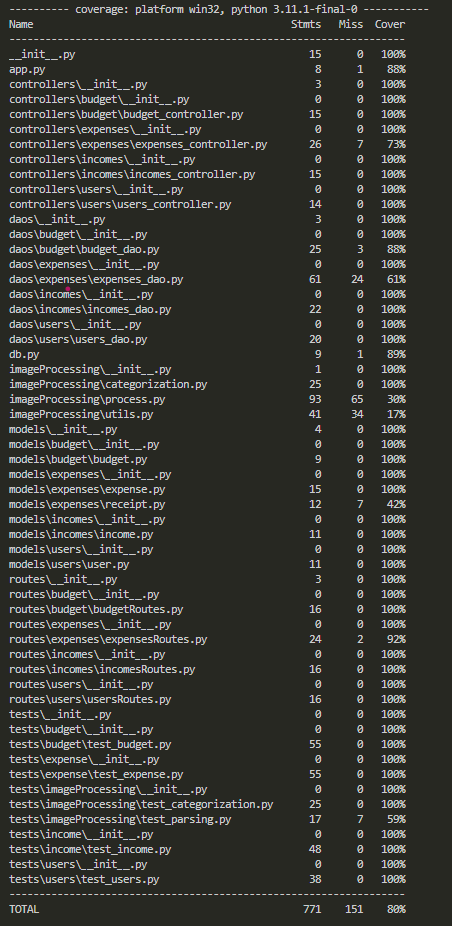
\includegraphics[width=\linewidth, height=0.85\textheight, keepaspectratio]{./coverage-backend.png}
  \caption{Backend Code Coverage Metrics}\label{fig:coverage-backend}
\end{figure}

\newpage{}

Frontend coverage metrics is calculated using Jest. See Figure \ref{fig:coverage-frontend}.
\begin{figure}[h!]
  \centering
  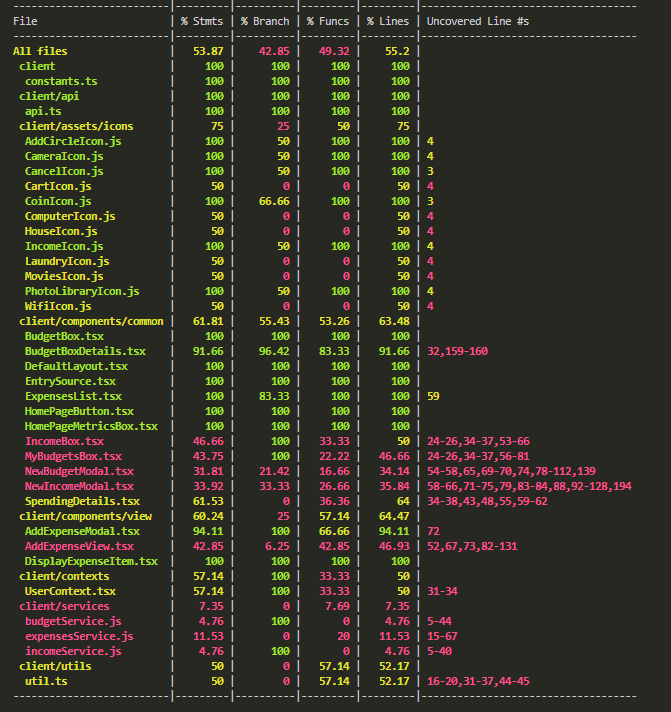
\includegraphics[width=\linewidth, height=0.85\textheight, keepaspectratio]{./coverage-frontend.png}
  \caption{Frontend Code Coverage Metrics}\label{fig:coverage-frontend}
\end{figure}
\newpage{}

\section*{Appendix --- Reflection}

The information in this section will be used to evaluate the team members on the
graduate attribute of Reflection.

The purpose of reflection questions is to give you a chance to assess your own
learning and that of your group as a whole, and to find ways to improve in the
future. Reflection is an important part of the learning process.  Reflection is
also an essential component of a successful software development process.  

Reflections are most interesting and useful when they're honest, even if the
stories they tell are imperfect. You will be marked based on your depth of
thought and analysis, and not based on the content of the reflections
themselves. Thus, for full marks we encourage you to answer openly and honestly
and to avoid simply writing ``what you think the evaluator wants to hear.''

Please answer the following questions.  Some questions can be answered on the
team level, but where appropriate, each team member should write their own
response:

\begin{enumerate}
  \item What went well while writing this deliverable? \\
  While writing the VnV report, it was noteworthy that the collaborative effort 
  among team members was highly effective. As we assigned each member a different
  area of testing, we ensured that the results brought into our meetings were insightful
  and understood by all of the other group members. This collaboration not only enhanced 
  the quality of the content but also ensured that all perspectives in response to the 
  feedback were considered. Finally, the thorough testing conducted prior to writing 
  the report provided a good foundation to plan out the future steps of development. 
  This allowed us to present concrete evidence of our findings, validating the findings 
  outlined in the report.
  \item What pain points did you experience during this deliverable, and how did you resolve them?\\
    One challenge we faced was managing all of the feedback received from Rev 0 as well 
    as the feedback provided from the users. There were some differing opinions as to how 
    we should address these responses moving forward. We held a meeting to discuss the 
    feedback together, allowing us to prioritize the most important points and agree on 
    how to approach them within our implementation. Another challenge was ensuring the 
    technical details, especially in the testing and results sections, were accurate. 
    Some team members had more knowledge of their assigned testing areas, which could 
    create gaps. To mitigate these gaps we had several meetings where team members shared 
    their expertise, helping improve our understanding and ensure the report was well written
    and that all group members had a solid understanding of all testing aspects.
  \item Which parts of this document stemmed from speaking to your client(s) or
  a proxy (e.g. your peers)? Which ones were not, and why?\\
  Several sections of the VnV report were shaped by feedback from clients and peers. 
  For example, the "Changes Due to Testing" section was influenced by the input provided by 
  the instructor and TA during the Rev 0 demo, which highlighted the need for better 
  usability features. This led us to adjust our focus to user-centered features. Peer reviews 
  also helped refine our assessment of functional and nonfunctional requirements.
  On the contrary, some parts of the report, like the technical details of testing methods 
  and code coverage metrics, were based on internal discussions and research. These sections 
  relied on our team's expertise and the VnV Plan, as they required a deeper understanding 
  of the system's technical aspects, while the feedback focused more on the project’s overall 
  direction.
  \item In what ways was the Verification and Validation (VnV) Plan different
  from the activities that were actually conducted for VnV?  If there were
  differences, what changes required the modification in the plan?  Why did
  these changes occur?  Would you be able to anticipate these changes in future
  projects?  If there weren't any differences, how was your team able to clearly
  predict a feasible amount of effort and the right tasks needed to build the
  evidence that demonstrates the required quality?  (It is expected that most
  teams will have had to deviate from their original VnV Plan.)\\
  The content of the VnV report differed from the original plan due to continuous feedback, 
  unforeseen technical challenges, and a greater emphasis on features revolving around usability. 
  We had to modify our approach by expanding user-focused testing, introducing additional test 
  cases, and addressing unexpected issues. These changes occurred as we gained new insights 
  and encountered limitations in our initial assumptions. To improve future planning, we can 
  allocate more buffer time, conduct early individual pilot tests for core functional features, and 
  allow for more flexibility in our initial VnV plan. Despite these deviations, our team 
  effectively adapted to ensure a thorough validation process with sufficient coverage to guide
  further development.
\end{enumerate}

\end{document}